\section{Methodology}\label{sec:methodology}
The goal of this section is to check if the aforementioned approach can consistently retrieve optimal decision tree policies for a simple grid world MDP (figure~\ref{fig:mdp-dt}).
In particular, we use reinforcement learning to train decision tree policies for MDPs by seeking deterministic memoryless policies that optimize the RL objective in POIBMDPs (figure~\ref{fig:ibmdp-example} and section~\ref{sec:poibmdp}).

\subsection{Computing some decision tree policies}
To assess the performance of reinforcement learning, for different trade-off reward $\zeta$ (definition~\ref{def:ibmdp}), we identify the deterministic memoryless policies that maximize the RL objective (definition~\ref{def:mdp-obj}). Each of those policies correspond to one of the decision tree policies for the grid world downstream MDP illustrated in figure~\ref{fig:irl-objectives}: (i) a depth-0 tree equivalent to always taking the same downstream action ($\pi_{\mathcal{T}_0}$), (ii) a depth-1 tree equivalent alternating between an IGA and a downstream action ($\pi_{\mathcal{T}_1}$), (iii) an unbalanced depth-2 tree that sometimes takes two IGAs then a downstream action and sometimes a an IGA then a downstream action ($\pi_{\mathcal{T}_u}$), (iv) a depth-2 tree that alternates between taking two IGAs and a downstream action ($\pi_{\mathcal{T}_2}$), or (v) an infinite `tree'' that only takes IGAs. We will particularly focus on trying to retrieve the depth-1 decision tree that is the most interpretable--smallest number of nodes and shallowest--tree taking optimal actions. Because from~\citet{learning-pomdp} we know that for POMDPs, stochastic memoryless policies can sometimes get better expected discounted rewards than deterministic memoryless policies, we also compute the value of the stochastic policy that randomly alternates between two downstream actions: $\rightarrow$ and $\downarrow$. Taking those two downstream actions always lead to the goal state in expectation (figure~\ref{fig:mdp-dt}). Because we know all the downstream states, all the observations, all the actions, all the rewards and all the transitions of our POIBMDPs, we can compute the RL objective values of those different deterministic memoryless policies exactly given $\zeta$ and $\gamma$ a discount factor. We plot, in figure~\ref{fig:irl-objectives}, the RL objective values of the decision tree policies as functions of $\zeta$ when we fix $\gamma=0.99$ (standard choice of discount in practice~\cite{sutton}). Despite objective values being very similar for the depth-1 and unbalanced depth-2 tree, we now know from the green shaded area that a depth-1 tree is optimal when $0< \zeta < 1$ in the POIBMDP. 
Interestingly, two challenges of learning in POMDPs described in~\cite{learning-pomdp} are visible in figure~\ref{fig:irl-objectives}. First, there is a whole range of $\zeta$ values for which the optimal memoryless policy is stochastic. Second, for e.g. $\zeta=0.5$, while the optimal deterministic memoryless policy corresponds to a depth-1 tree, the value of the (PO)IBMDP state $(\boldsymbol{s}_2, \boldsymbol{o}_0) = (1.5, 1.5, 0, 2, 0, 2)$, i.e. the agent current position is upper right cell in the downstream MDP but it has not information about it, is not maximized by the optimal memoryless policy that will take 1 information-gathering action in between each downstream action (figure~\ref{fig:irl-objectives}), but by the sub-optimal policy that always goes down. Next, we present the specific experimental setup that we use in the remaining of the paper.
\begin{figure*}
    \begin{subfigure}{0.55\textwidth}
    \centering
    \scalebox{0.55}{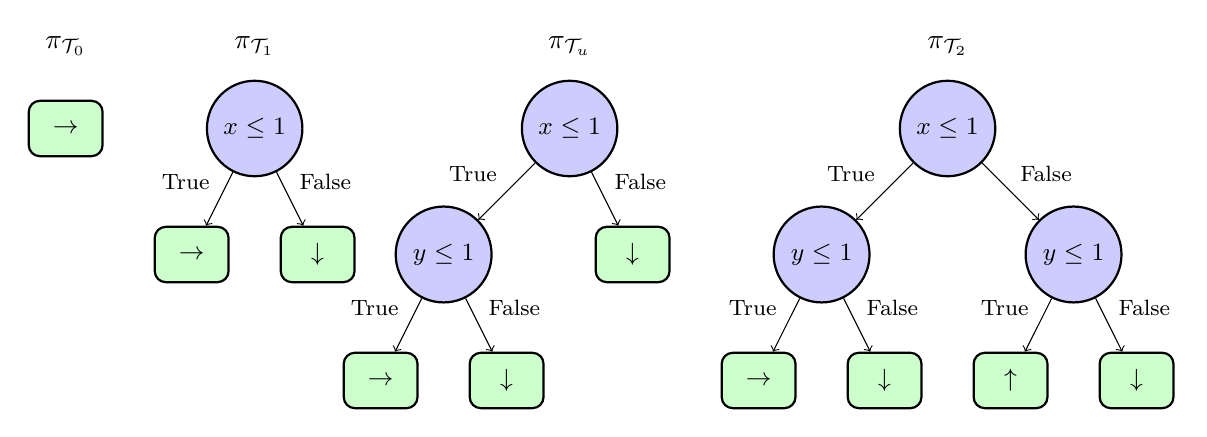
\begin{tikzpicture}[
        scale=0.8,
        decision/.style={circle, draw, thick, fill=blue!20, text width=2.5em, text centered, minimum height=2.5em, font=\small},
        leaf/.style={rectangle, draw, thick, fill=green!20, text width=2em, text centered, rounded corners, minimum height=2em, font=\small},
        edge_label/.style={font=\footnotesize, midway}
    ]
        
        \node[leaf] at (-3, 0) {$\rightarrow$};
        % Tree 4: if x <= 0.5 move right else move left
        \node[decision] (tree4_root) at (0,0) {$x \leq 1$};
        \node[leaf] (tree4_right) at (-1,-2) {$\rightarrow$};
        \node[leaf] (tree4_left) at (1,-2) {$\downarrow$};
        \draw[->] (tree4_root) -- (tree4_right) node[edge_label, above left] {True};
        \draw[->] (tree4_root) -- (tree4_left) node[edge_label, above right] {False};
        
        % Draw a square around the tree
        % \draw[thick, red] (-2, 1.8) rectangle (2, -2.5);

        % Tree 7: if x <= 0.5 and y <= 0.5 move right else move down
        \node[decision] (tree7_root) at (5,0) {$x \leq 1$};
        \node[decision] (tree7_y) at (3,-2) {$y \leq 1$};
        \node[leaf] (tree7_right) at (2,-4) {$\rightarrow$};
        \node[leaf] (tree7_down) at (4,-4) {$\downarrow$};
        \node[leaf] (tree7_down2) at (6,-2) {$\downarrow$};
        \draw[->] (tree7_root) -- (tree7_y) node[edge_label, above left] {True};
        \draw[->] (tree7_root) -- (tree7_down2) node[edge_label, above right] {False};
        \draw[->] (tree7_y) -- (tree7_right) node[edge_label, above left] {True};
        \draw[->] (tree7_y) -- (tree7_down) node[edge_label, above right] {False};


        \node[decision] (tree7_root) at (11,0) {$x \leq 1$};
        \node[decision] (tree7_y) at (9,-2) {$y \leq 1$};
        \node[decision] (tree7_y2) at (13,-2) {$y \leq 1$};
        \node[leaf] (tree7_right) at (8,-4) {$\rightarrow$};
        \node[leaf] (tree7_down) at (10,-4) {$\downarrow$};
        \node[leaf] (tree7_right2) at (12,-4) {$\uparrow$};
        \node[leaf] (tree7_down2) at (14,-4) {$\downarrow$};
        \draw[->] (tree7_root) -- (tree7_y) node[edge_label, above left] {True};
        \draw[->] (tree7_root) -- (tree7_y2) node[edge_label, above right] {False};
        \draw[->] (tree7_y) -- (tree7_right) node[edge_label, above left] {True};
        \draw[->] (tree7_y) -- (tree7_down) node[edge_label, above right] {False};
        \draw[->] (tree7_y2) -- (tree7_right2) node[edge_label, above left] {True};
        \draw[->] (tree7_y2) -- (tree7_down2) node[edge_label, above right] {False};

        % Labels
        \node[above] at (-3,1) {$\pi_{\mathcal{T}_0}$};
        \node[above] at (0,1) {$\pi_{\mathcal{T}_1}$};
        \node[above] at (5,1) {$\pi_{\mathcal{T}_u}$};
        \node[above] at (11,1) {$\pi_{\mathcal{T}_2}$};


    \end{tikzpicture}}
\end{subfigure}
\hfill
\begin{subfigure}{0.45\textwidth}
    \centering
    \includegraphics[width=0.95\textwidth]{../images/images_part1/objective_values_plot.pdf}
\end{subfigure}
\caption{Decision tree policies and their RL objective values (definition~\ref{def:mdp-obj}) as functions of the rewards $\zeta$ in POIBMDPs associated to the grid world MDP (figure~\ref{fig:ibmdp-example}). Shaded areas on the right plot indicate which deterministic memoryless policy is optimal depending on $\zeta$.
Recall that $\zeta$ can be seen as a reward that encourages the deterministic memoryless policy to take information-gathering actions, i.e. the reward that trades off interpretability of the corresponding decision tree and its cumulative reward.}\label{fig:irl-objectives}
\end{figure*}

\subsection{Experimental setup}
All our code is open source\footnote{\url{https://anonymous.4open.science/r/poibmdps-5BFE/}}.
The downstream MDP for which we want to learn decision tree policies with reinforcement learning is the grid world MDP (figure~\ref{fig:mdp-dt}).
We then get 100 associated POIBMDPs following figure~\ref{fig:ibmdp-example} with $\zeta$ chosen uniformly among 100 different in $]0, 1[$. 

We will evaluate two types of reinforcement learning algorithm.
Frist we use standard tabular RL algorithms, namely Q-learning, Sarsa, and vanilla policy gradient on a softmax policy~\cite{watkins1992q,sutton,jsj}, to learn deterministic memoryless policies in POIBMDPs by simply replacing the current state in the algorithm descriptions by the current observation.
In theory the policy gradient algorithm should not be a good candidate for our problem since it searches for stochastic policies that we showed can be better than our sought depth-1 decision tree policy (figure~\ref{fig:irl-objectives}), but for completeness we will see what trees are obtained after greddification of the stochastic policies.

Second, we also use the more specialised asymmetric Q-learning, asymmetric Sarsa, and asymmetric policy gradient (algorithm~\ref{alg:asymqlearning}, section~\ref{sec:asym}).
Each algorithm is trained until convergence on each POIBMDP, and each one of those runs is repeated 100 times.
For all baselines we use, when applicable, exploration rates $\epsilon=0.3$ and learning rates $\alpha=0.1$.
All the training curves are presented in appendix~\ref{sec:training}.

We will consider two metrics.
We consider the distribution of the learned trees over the 100 training seeds.
Indeed, since for every POIBMDP we run each algorithm 100 times, at the end of training we get 100 deterministic memoryless policies, from which we can extract the equivalent 100 decision tree policies using algorithm~\ref{alg:extract-tree} and we can count which one have e.g. a depth of 1.
This helps understand which trees RL algorithms tend to learn as a function of the trade-off reward $\zeta$.


\subsection{Can reinforcement learning find the optimal deterministic memoryless POIBMDP policies?}\label{sec:experiments}

In figure~\ref{fig:dt-distrib-poibmdp}, we plot the distributions of the final learned trees over the 100 random seeds in function of $\zeta$ from the above runs.
For example, in figure~\ref{fig:dt-distrib-poibmdp}, in the top left plot, when learning 100 times in a POIBMDP with $\zeta=0.5$, Q-learning returned almost 100 times a depth-0 tree.
Again, on none of those subplots do we see a high rate of learned depth-1 trees for $\zeta\in ]0, 1[$.
It is alerting that the most frequent learned trees are the depth-0 trees for $\zeta\in ]0, 1[$ because such trees are way more sub-optimal than e.g. the depth-2 unbalanced trees (figure~\ref{fig:irl-objectives}).  
One interpretation of this phenomenon is that the learning in POIBMDPs is very difficult and so agents tend to converge to trivial policies, e.g., repeating the same downstream action.
Furhtermore, in appendix~\ref{sec:training} we show that for POIBMDPs with $\zeta \in [-1, 0]$ and $\zeta \in [1, 2]$, baselines consistently learn the optimal policies--a depth-0 tree and an infinite tree respectively--which is concerning as it means that RL seem to find only trivial policies.
On the positive side, we observe that asymmetric versions of Q-learning and Sarsa have found the optimal deterministic memoryless policy--the depth-1 decision tree--more frequently throughout the optimality range $]0,1[$, than their symmetric counter-parts for $\zeta\in ]0, 1[$.
Next, we quantify how difficult it is to do RL to learn memoryless policies in POIBMDPs as opposed to standard Markovian polciies.

\begin{figure}
    \centering
    \includegraphics[width=0.4\textwidth]{../slides_soutenance/tree_distributions.pdf}
    \caption{Distributions of final tree policies learned across the 100 seeds.
    For each $\zeta$ value, there are four colored points. Each point represent the share of depth-0 trees (red), depth-1 trees (green), unbalanced depth-2 trees (orange) and depth-2 trees (blue).
    }\label{fig:dt-distrib-poibmdp}
\end{figure}


\subsection{How difficult is it to learn in POIBMDPs?}\label{sec:how-diff}

In this section we run the same (asymmetric) reinforcement learning algorithms to learn standard Markovian policies in MDPs (definition~\ref{def:mdp}) or IBMDPs (definition~\ref{def:ibmdp}), or deterministic memoryless policies in POIBMDPs (definition~\ref{def:poibmdp}).

In order to see how difficult each of these three problems is, we can run a \textit{great} number of experiments for each problem and compare solving rates.
To make solving rates comparable we consider a unique instance for each of those problems.
Problem 1 is learning one of the optimal standard Markovian deterministic policy ($\pi: S\rightarrow A$)from figure~\ref{fig:mdp-dt} for the grid world MDP with $\gamma=0.99$.
Problem 2 is learning one of the optimal standard Markovian deterministic policy ($\pi: S\times O \rightarrow A \cup A_{info}$) for the IBMDP from figure~\ref{fig:ibmdp-example} with $\gamma=0.99$ and $\zeta=0.5$.
Problem 3 is what has been done in the previous section to learn deterministic memoryless policies ($\pi: O \rightarrow A \cup A_{info}$) where in addition of fixing $\gamma=0.99$ we also fix $\zeta=0.5$.

We use the six (asymmetric) RL algorithms from the previous section and try a wide set of hyperparameters and additional learning tricks (optimistic Q-function, eligibility traces, entropy regularization and $\epsilon$-decay, all are described in \cite{sutton}).
The complete detailed lists of hyperparameters are given in the appendix~\ref{sec:hp-pomdp} and a summary is given in table~\ref{tab:ib-params}.
Furthermore, the careful reader might notice that there is no point running asymmetric RL on MDPs or IBMDPs when the problem does not require partial observability.
Hence, we only run asymmetric RL for POIBMDPs and otherwise run all other RL algorithms and all problems.

Each unique hyperparameter combination for a given algorithm on a given problem is run 10 times on 1 million learning steps to get standard errors.
For example, for asymmetric Sarsa, we run a total of $10\times 768= 7680$ experiments for learning deterministic memoryless policies for a POIBMDP.
To get a success rate, we can simply divide the number of learned optimal depth-1 tree by 768 (recall that for $\gamma=0.99$ and $\zeta=0.5$, the optimal policy is a depth-1 tree (e.g. figure~\ref{fig:irl-objectives}). 


The key observations from figure~\ref{fig:po-vs-ib} is that reinforcement learning a deterministic memoryless policy in a POIBMDP, is way harder than learning a standard Markovian policy.
For example, Q-learning finds the optimal solution in only 3\% of the experiments while the same algorithms to optimize the standard RL objective (definition~\ref{def:mdp-obj}) in an MDP or IBMDP found the optimal solutions 50\% of the time.
Even though asymmetry seems to increase performances; learning a decision tree policy for a simple grid world directly with RL using the framework of POIBMDP originally developed in~\citet{topin2021iterative} seems way too difficult and costly as successes might require a million steps for such a seemingly simple problem.
An other difficulty in practice that we did not cover here, is the choice of information gathering actions.
For the grid world MDP, choosing good IGAs ($x\leq1$ and $y\leq1$) is simple but what about more complicated MDPs: how to instantiate the (PO)IBMDP action space such that internal nodes in resulting trees are useful for predictions?
Next, we further support that partial observability is the main limitation for reinforcement learning to train decision tree policies for MDPs.

\begin{figure}
    \centering
    \includegraphics[width=0.4\textwidth]{../slides_soutenance/barplot_with_std.pdf}
    \caption{Success rates of different (asymmetric) RL algorithms over thousands of runs when applied to learning deterministic memoryless policies in a POIBMDP or learning deterministic policies in associated MDP and IBMDP.}\label{fig:po-vs-ib}
\end{figure}

\subsection{Are they downstream MDPs for which partial observability is not a limitation?}
In this section, we show that for a special class of POIBMDPs, reinforcement learning can learn optimal deterministic memoryless policies w.r.t the RL objective, i.e. we can do direct decision tree policy learning for MDPs.
This class of POIBMDPs are those for which downstream MDPs have uniform transitions, i.e. $T(\boldsymbol{s}, a, \boldsymbol{s}') = \frac{1}{|S|}$ (definitions~\ref{def:mdp} and~\ref{def:ibmdp}).
Such downstream MDPs include classification tasks formulated as MDPs.
This implies that learning deterministic memoryless policies in POIBMDPs where the downstream MDP encodes a classification task is equivalent to doing supervised learning of a decision tree (figure~\ref{example:cmdp}).
This is exactly what is done in e.g.~\citet{dpdt}.
In figure~\ref{example:cmdp} we give an example of such downstream MDPs for a classification task with 4 data in the training set and 2 classes: $\mathcal{X} = \{(0.5, 0.5), (0.5, 1.5), (1.5, 1.5), (1.5, 0.5)\}$ and $y = \{0, 0, 1, 1\}$.

In appendix~\ref{sec:classif}, we show that POIBMDPs associated to downstream MDPs with uniform transitions are themselves standard MDP (definition~\ref{def:mdp}).
This means that in principle, standard RL algorithms like Q-learning, should work as well as for any MDP.
If RL does work for such fully observable POIBMDPs, this would mean that the difficulty of direct learning of decision tree policies for \textit{any} MDP using POIBMDPs, exhibited in sections, is most likely due to the partial observability.
This is exactly what we check next.
We use the same direct approach to learn decision tree policies as in previous sections, except that now the downstream MDP is a classification task and not a sequential decision making task like reaching a goal in a grid world.

We construct POIBMDPs for the classification task from figure~\ref{example:cmdp}, with $\gamma=0.99$, 200 values of $\zeta \in [0,1]$ and IGAs $x\leq 1$ and $y\leq 1$.
Since those POIBMDPs are MDPs, we do not need to analyze asymmetric RL baselines.
We see on figure~\ref{fig:tree-distrib-classif-poibmdp} that compared to general POIBMDPs from previous sections, RL can be used to consistently learn optimal deterministic memoryless policies $O:\rightarrow A\cup A_{info}$.
Such policies are equivalent to decision tree classifiers.

\begin{figure}
    \centering
    \scalebox{0.8}{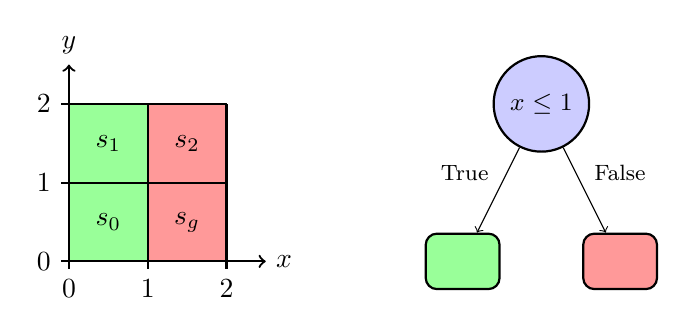
\begin{tikzpicture}[
        decision/.style={circle, draw, thick, fill=blue!20, text width=2.5em, text centered, minimum height=2.5em, font=\small},
        leaf/.style={rectangle, draw, thick, fill=green!20, text width=2em, text centered, rounded corners, minimum height=2em, font=\small},
        edge_label/.style={font=\footnotesize, midway}
    ]
        % Tree 4: if x <= 0.5 move right else move left
        \node[decision] (tree4_root) at (6,2) {$x \leq 1$};
        \node[rectangle, draw, thick, fill=green!40, text width=2em, text centered, rounded corners, minimum height=2em, font=\small] (tree4_right) at (5,0) {};
        \node[rectangle, draw, thick, fill=red!40, text width=2em, text centered, rounded corners, minimum height=2em, font=\small] (tree4_left) at (7,0) {};
        \draw[->] (tree4_root) -- (tree4_right) node[edge_label, above left] {True};
        \draw[->] (tree4_root) -- (tree4_left) node[edge_label, above right] {False};
        \tikzstyle{grid}=[draw, thick, fill=gray!10]
        
        % Draw grid
        \draw[fill=green!40] (0, 0) rectangle (1,2);
        \draw[fill=red!40] (1, 0) rectangle (2,2);

        \draw[grid] (0,0) grid (2,2);
        
        % Add axes
        \draw[thick, ->] (0,0) -- (2.5,0) node[right] {$x$};
        \draw[thick, ->] (0,0) -- (0,2.5) node[above] {$y$};
        
        % Add tick marks and labels
        \foreach \x in {0,1,2} {
            \draw[thick] (\x,0) -- (\x,-0.1) node[below] {$\x$};
        }
        \foreach \y in {0,1,2} {
            \draw[thick] (0,\y) -- (-0.1,\y) node[left] {$\y$};
        }

        \node at (0.5,0.5) {$\boldsymbol{s}_0$};
        \node at (1.5,0.5) {$\boldsymbol{s}_g$};
        \node at (1.5,1.5) {$\boldsymbol{s}_2$};
        \node at (0.5,1.5) {$\boldsymbol{s}_1$};

    \end{tikzpicture}}
    \caption{In this MDP, there are four data to which to assign either a green or red label.
    On the right, there is the unique optimal depth-1 tree for this particular MDP. This depth-1 tree also maximizes the accuracy on the corresponding classification task.}\label{example:cmdp}
    \end{figure}

\begin{figure}
    \centering
    \includegraphics[width=0.4\textwidth]{../slides_soutenance/tree_distributions_merged.pdf}
    \caption{We reproduce the same plot as in figure~\ref{fig:dt-distrib-poibmdp} for POIBMDPs associated to a downstream MDP encoding a classification task. Each colored dot is the number of final learned trees with a specific structure for a given $\zeta$.}\label{fig:tree-distrib-classif-poibmdp}
\end{figure}